\newpage
\section{Analiza problemu}		%2
%Napisać gdzie używa się tego algorytmu
%Opisać sposób działania programu/algorytmu
%Napisać spsoób wykorzystania algorytmu po przez wykonanie przykładu (np. mnożenie macierzy - wykonać ręcznie przykład z mnożeniem macierzy pokazujący jak mnoży się macierz ręcznie)
\hspace{0.60cm}Lista dwukierunkowa jest to struktura danych po której możemy poruszać się w dwóch kierunkach, do przodu i do tyłu. Każdy element zawiera wskaźnik na poprzedni (prev) lub następny (next) element w liście oraz dane (data) Rys. \ref{rys:rysunek001} (s. \pageref{rys:rysunek001}).

\begin{figure}[!htb]
	\begin{center}
		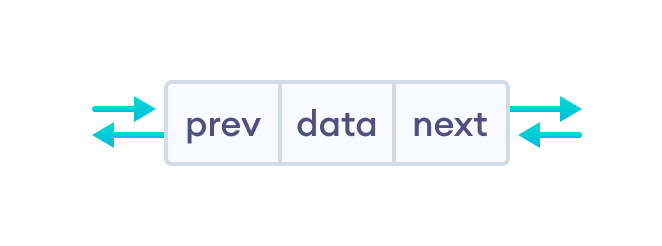
\includegraphics{Dokumentacja/rys/lista.png}
		\caption{Element listy.\footnotemark}
		\label{rys:rysunek001}
	\end{center}
\end{figure}

\footnotetext{\label{note1}Infografika ze strony https://www.programiz.com/dsa/doubly-linked-list\cite{www1}.}

\hspace{0.60cm}Na liście dwukierunkowej można przeprowadzać wiele operacji, takich jak dodawanie elementu na początek listy. Polega ono na połączeniu ze sobą wskaźnika next nowo stworzonego elementu ze wskaźnikiem prev elementu z początku listy (head) w taki sposób aby na siebie wskazywały Rys. \ref{rys:rysunek002} (s. \pageref{rys:rysunek002}).

\begin{figure}[!htb]
	\begin{center}
		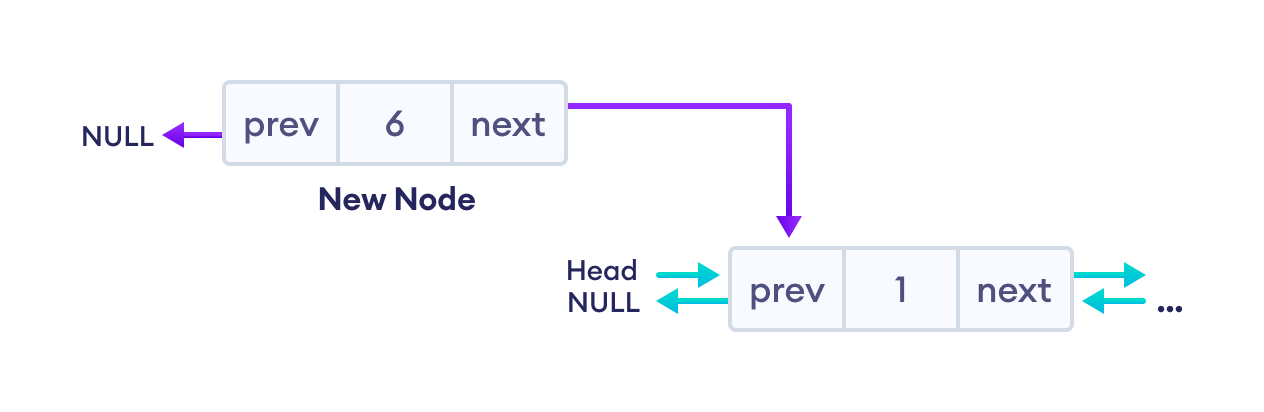
\includegraphics[scale=0.7]{Dokumentacja/rys/dodaj_na_poczatek.png}
		\caption{Dodawanie elementu na początek.\footref{note1}}
		\label{rys:rysunek002}
	\end{center}
\end{figure}

\newpage

\hspace{0.60cm}Kolejną operacją jest dodanie elementu na koniec. Przebiega ona podobnie jak z dodawaniem na początek z róźnicą, że łączymy ostatni element (tail) z nowo stworzonym Rys. \ref{rys:rysunek003} (s. \pageref{rys:rysunek003}).

\begin{figure}[!htb]
	\begin{center}
		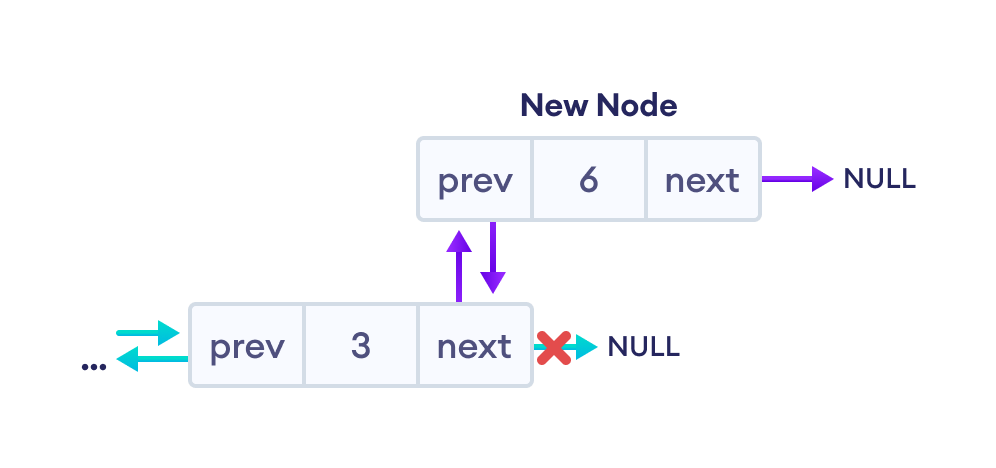
\includegraphics[scale=0.7]{Dokumentacja/rys/dodaj_na_koniec.png}
		\caption{Dodawanie elementu na koniec.\footref{note1}}
		\label{rys:rysunek003}
	\end{center}
\end{figure}

\footnotetext{\label{note1}Infografika ze strony https://www.programiz.com/dsa/doubly-linked-list\cite{www1}.}

\hspace{0.60cm}Możemy także wstawić element pod wskazany indeks łącząc ze sobą wskaźnik prev nowego elemnentu z wskaźnikiem next poprzedzającego indeks Rys. \ref{rys:rysunek004} (s. \pageref{rys:rysunek004}) oraz wskaźnik next z wskaźnikiem prev następnego po wskazanym indeksie Rys. \ref{rys:rysunek005} (s. \pageref{rys:rysunek005}).

\begin{figure}[!htb]
	\begin{center}
		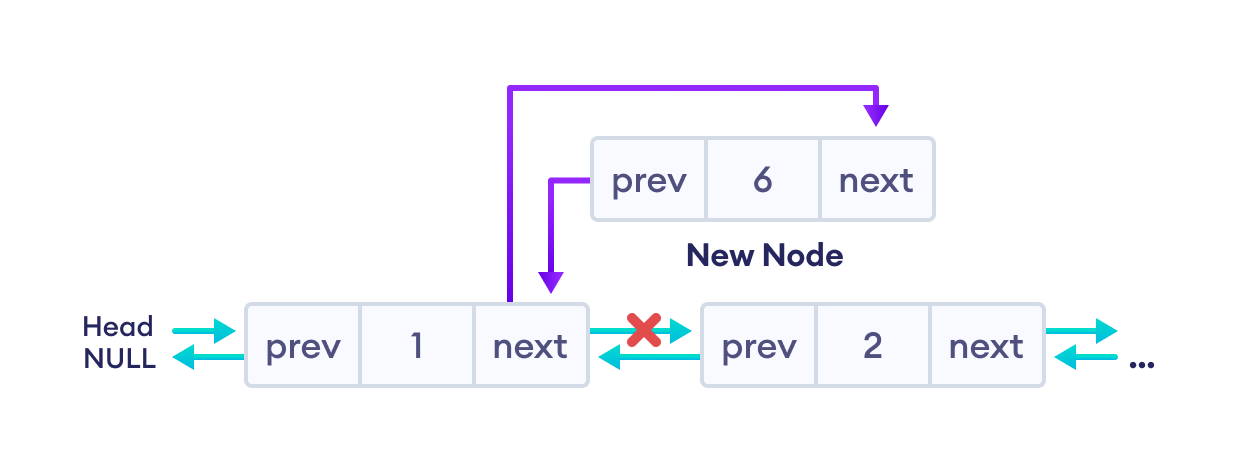
\includegraphics[scale=0.7]{Dokumentacja/rys/dodaj_indeks1.png}
		\caption{Łączenie z poprzedzającym elementem.\footref{note1}}
		\label{rys:rysunek004}
	\end{center}
\end{figure}

\newpage

\begin{figure}[!htb]
	\begin{center}
		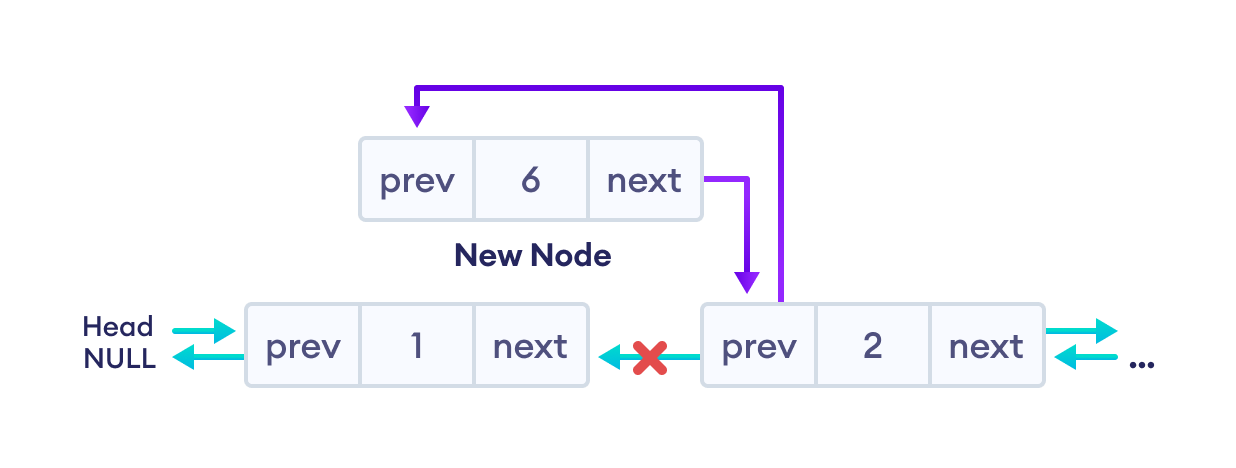
\includegraphics[scale=0.7]{Dokumentacja/rys/dodaj_indeks2.png}
		\caption{Łączenie z następnym elementem.\footref{note1}}
		\label{rys:rysunek005}
	\end{center}
\end{figure}

\footnotetext{\label{note1}Infografika ze strony https://www.programiz.com/dsa/doubly-linked-list\cite{www1}.}

\hspace{0.60cm}W analogiczny sposób przeprowadza się operację usuwania elementów z listy dwukierunkowej. Pierwszy i ostatni element usuwa się poprzez wpisywanie wartości NULL, żeby na nic nie wskazywały, do wskaźników elementów head i tail \ref{rys:rysunek006} i \ref{rys:rysunek007} (s. \pageref{rys:rysunek006}). Inaczej wygląda usuwanie wybranego elementu, gdzie łączy się ze sobą wskaźniki poprzedzającego i następującego elementu aby ten, którego chcemy się pozbyć nie należał już do listy \ref{rys:rysunek008} (s. \pageref{rys:rysunek008}).

\begin{figure}[!htb]
	\begin{center}
		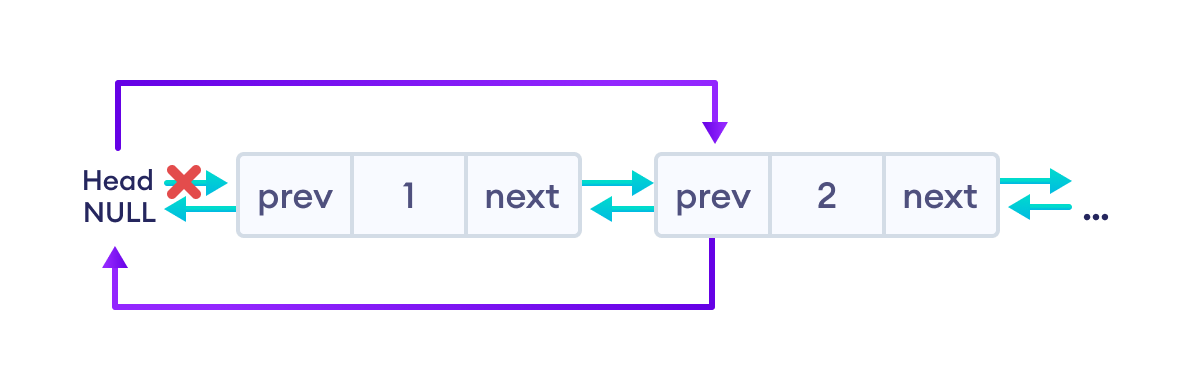
\includegraphics[scale=0.6]{Dokumentacja/rys/usun_przod.png}
		\caption{Usuwanie pierwszego elementu.\footref{note1}}
		\label{rys:rysunek006}
	\end{center}
\end{figure}

\begin{figure}[!htb]
	\begin{center}
		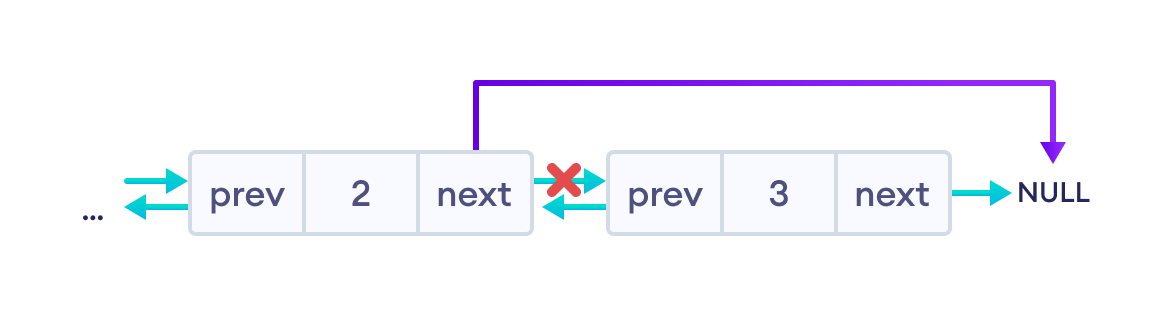
\includegraphics[scale=0.6]{Dokumentacja/rys/usun_koniec.png}
		\caption{Usuwanie ostatniego elementu.\footref{note1}}
		\label{rys:rysunek007}
	\end{center}
\end{figure}

\newpage

\footnotetext{\label{note1}Infografika ze strony https://www.programiz.com/dsa/doubly-linked-list\cite{www1}.}

\begin{figure}[!htb]
	\begin{center}
		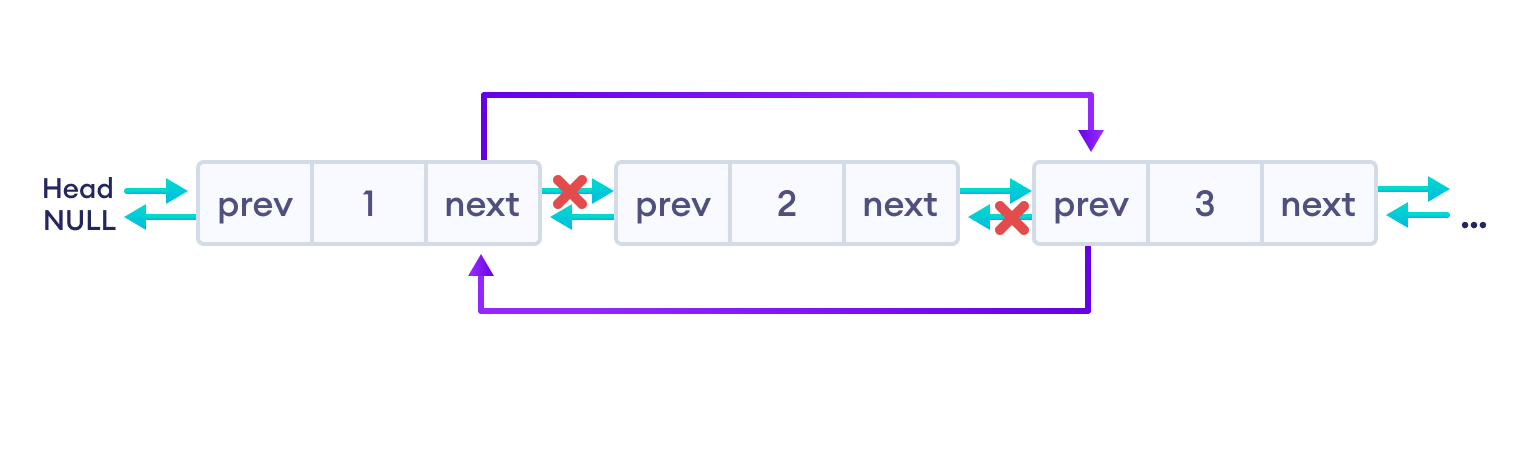
\includegraphics[scale=0.5]{Dokumentacja/rys/usun_srodek.png}
		\caption{Usuwanie wybranego elementu.\footref{note1}}
		\label{rys:rysunek008}
	\end{center}
\end{figure}
